\documentclass[review]{elsarticle}

\usepackage{lineno,hyperref}
\usepackage{xcolor}
\usepackage[labelfont=bf]{caption}
\modulolinenumbers[5]

\journal{Journal of Information Processing and Management }

\bibliographystyle{elsarticle-num}

\newcommand{\beginsupplement}{%
        \setcounter{table}{0}
        \renewcommand{\thetable}{S\arabic{table}}%
        \setcounter{figure}{0}
        \renewcommand{\thefigure}{S\arabic{figure}}%
     }

\begin{document}

\begin{frontmatter}

\title{Investigating Facebook's actions against accounts that repeatedly share misinformation}

\author[mymainaddress]{Héloïse Théro\corref{mycorrespondingauthor}}
\cortext[mycorrespondingauthor]{Corresponding authors.}
\ead{thero.heloise@gmail.com}

\author[mymainaddress]{Emmanuel M. Vincent\corref{mycorrespondingauthor}}
\ead{emmanuel.vincent@sciencespo.fr}

\address[mymainaddress]{médialab - Sciences Po, Paris, France}

\begin{abstract}

Like many web platforms, Facebook is under pressure to regulate misinformation.
According to the company, users that repeatedly share misinformation (`repeat offender') will have their distribution reduced, but little is known about the implementation or the efficiency of this measure.
First, combining data from a fact-checking organization and CrowdTangle, we identified a set of public accounts (groups and pages) that have shared misinformation repeatedly during the 2019-2020 period.
While we observe a decrease in engagement for pages after they shared two or more `false news', such a reduction is not observed for `repeat offender' groups.
This result was replicated using a more complete set of misinformation URLs shared by Facebook (Condor data).
We also discover that groups have been affected in a different way with a sudden drop in their average engagement per post that occurred around June 9, 2020.
Finally we identified a set of pages claiming to be put under `reduced distribution' by Facebook for repeatedly sharing misinformation, and we again observed a decrease in their engagement per post.
In the three sets of pages studied, the median decrease in engagement after sharing misinformation is ranging from $-62\%$ to $-24\%$.
Our results highlight easy steps Facebook could take to reduce misinformation, such as to enforce their `repeat offender' policy more forcefully on pages, and to start applying it to groups.

\end{abstract}

\begin{keyword}
Misinformation\sep Content moderation\sep Algorithmic transparency\sep Facebook\sep Fact-checking\sep Social media analysis
%\MSC[2010] 00-01\sep  99-00
\end{keyword}

\end{frontmatter}

\linenumbers

\section{Introduction}

The general public is increasingly getting news related information online, through search engines, social media and video platforms \citep{mitchell2016modern}.
Hence the spread of misinformation through these platforms has recently received growing attention.
Recent studies, along with the political context of January 2021 in the United States, show how the presence of misinformation online can contribute to negative societal consequences.
Namely it can fuel false beliefs, such as the idea of a massive voter fraud during the US 2020 presidential election, which may have led to the January 6, 2021 insurrection at the U.S. Capitol \citep{benkler2020mail} and other false stories about presidential candidates \citep{allcott2017social}. 
Misinformation has also confused the public about the reality of climate change \citep{brulle30years, porter2019can} and stoked skepticism about vaccine safety among the public \citep{featherstone2020feeling, lahouati2020spread}. 
In April 2020, a questionnaire from the Reuters Institute found that people in the UK use online sources more often than offline sources when looking for information about the coronavirus. 
Among social media platforms, Facebook was the most widely used with $24\%$ of the respondents saying they used Facebook to access COVID-19 information in the last seven days \citep{fletcher2020information}.
The importance of Facebook in the media landscape is confirmed by Parse.ly’s dashboard, which shows that $25\%$ of the visitors of 2500+ media websites are referred by Facebook \citep{parslyDashboard}.

Lawmakers and regulators are increasingly pressuring platforms to limit the spread of misinformation. 
In the US, the House of Representatives organized hearings and convened representatives of the main platforms to testify on how they are being weaponized to spread ``misinformation and conspiracy theories online'' \citep{donovan2020}. 
In Europe, the European Commission has established a `Code of Practice on Disinformation' \citep{codePracticeMisinformation} that enjoins platforms to voluntarily comply with a set of commitments \citep{heldt2019let}. 
However, there is little data available and few established processes to monitor the implementation of these measures and quantify their actual impact. 
Here we propose a methodology to monitor Facebook’s implementation of its policy to reduce the visibility of accounts repeatedly spreading misinformation. 
We chose to focus on Facebook as it is the biggest social media platform with more than two billion users worldwide.

Facebook announced a three-part policy to address ‘misleading or harmful content’: they claim to \textit{remove} harmful information, \textit{reduce} the spread of misinformation and \textit{inform} people with additional context \citep{threePartRecipe}. 
Facebook has developed the most extensive third-party fact-checking program with dozens of partner institutions to assist the company in this endeavour \citep{60factCheckingPartners}.
Facebook informs page or group owners when published posts on their pages or groups are marked as misinformation, inviting them to correct the posts.
Facebook also states that the virality of the posts marked as `False' or `Partly False' will be reduced.

Facebook’s \textit{reduce} policy is not only applied to individual posts, but also to organizations and communities that often publish posts containing misinformation, as indicated by this statement in their publishers’ help center \citep{factCheckingRules, repeatOffenderCommunication}: 
\begin{quote}
\emph{Pages and websites that repeatedly share misinformation rated False or Altered will have some restrictions, including having their distribution reduced.}
\end{quote}
Facebook ranks each post by assigning to it a relevancy score, where a high score leads to a high likelihood of the post to appear on a user's newsfeed. 
Doing so, Facebook can make a post or a whole account less visible by decreasing the relevancy score of its content; this is precisely the {\it reduce} measure \citep{threePartRecipe}.

So far Facebook has not provided data showing how their {\it reduce} policy is implemented, which would allow researchers to quantify its impact on the spread of misinformation. 
To the best of our knowledge, the impact of the {\it reduce} policy has not yet been audited directly.
Hence the present research article departs from articles studying the overall levels of misinformation on platforms \citep{allcott2019trends, kornbluh2020new, resnick2018iffy}, by focusing on monitoring a specific policy against misinformation.

We used CrowdTangle, a public insights tool owned and operated by Facebook, to access Facebook data \citep{team2020crowdtangle}. 
CrowdTangle exclusively tracks public content, and provides access to engagement metrics (such as the number of likes, shares and comments), but not to the reach (number of views) of content \citep{helpCT}.
To investigate the effect of the reduce policy, we thus analyzed the engagement per post received by `repeat offender' accounts. 
Indeed, one would expect this metric to decline if the accounts’ posts become less visible in Facebook’s feed.
 
We first combined data from one of Facebook's fact-checking partners (Science Feedback) identifying URLs sharing misinformation and from CrowdTangle tracking engagement metrics of the Facebook accounts that repeatedly shared such misinformation.
We then replicated this methodology using a more complete source of misinformation URLs obtained directly from Facebook (Condor data).
Using another method to identify `repeat offender' accounts, we finally studied the engagement metrics of a set of Facebook pages claiming to be under reduced distribution.


\section{Research questions}

\begin{itemize}
\item Was the policy aiming to reduce the distribution of misinformation repeat offenders actually enforced by Facebook during the 2019-2020 period?
\item If so, what was the magnitude of the reduction applied? And is there a difference between Facebook groups and Facebook pages?
\item Does this action have an impact on the spread of misinformation on Facebook, i.e., can we see a global increase or decrease in engagement for the repeat offender accounts through time?
\end{itemize}

\section{Investigating the reduce policy on Facebook accounts repeatedly sharing misinformation (Science Feedback data)}

We used data from Science Feedback, which is part of Facebook’s third-party fact-checking program \cite{sciencefeedbackFbPartner}. 
Science Feedback is a fact-checking organization, where academics review the credibility of science-related claims and articles.

\subsection{Methods}

We obtained from Science Feedback a list of 4,000+ URLs reviewed by its team. 
We relied on the 2,452 URLs marked as `False', which we refer to as `false news links', excluding the URLs marked as `Partly False', `Missing Context', `False headlines' or `True', as well as the URLs marked as `False' but `corrected' by the publisher, because these labels do not contribute to the `repeat offender' status according to Facebook's guidelines.
Sharing a URL fact-checked as `Altered' also contribute to the `repeat offender' status \citep{factCheckingRules, repeatOffenderCommunication}, but we found no such rating in the Science Feedback data.
The list of `false news links' was obtained on January 4, 2021 and cover links flagged in 2019 and 2020.

Using the `/links' endpoint from the CrowdTangle API, we collected the public Facebook groups and pages that shared at least one false news link between January 1, 2019 and December 31, 2020. 
Due to the API limitations, if a URL was shared in more than 1000 posts, we collected only the 1000 posts that received the highest number of interactions \cite{docCT}. 
We focused on the accounts that spread misinformation the most often, choosing a threshold of 24 different false news links shared over the past two years.  

The corresponding 307 Facebook accounts (289 Facebook groups and 18 Facebook pages) are referred to as `repeat offenders accounts'. 
All the posts they published between January 1, 2019 and December 31, 2020 were collected using the `/posts' endpoint. 
We calculated the engagement per post by summing the number of comments, shares and reactions (such as ‘like’, ‘love’, ‘favorite’, ‘haha’, ‘wow’, ‘sad’ and ‘angry’ reactions) that each post has received.

`Repeat offender' accounts are supposed to have their distribution reduced, according to Facebook's official communication, but the precise rule Facebook uses to classify an account as `repeat offender' is not specified. 
However, an undisclosed source obtained by a journalist \cite{2strikes90daysRule} indicated that:
\begin{quote}
\emph{The company operates on a `strike' basis, meaning a page can post inaccurate information and receive a one-strike warning before the platform takes action. 
Two strikes in 90 days places an account into `repeat offender' status.}
\end{quote}


Based on this `two strikes in 90 days' rule and the list of strike dates known by Science Feedback, we inferred periods during which each account must have been under repeat offender status. 
If a post shares a misinformation link which was previously fact-checked as `False', we used the date of the post as the strike date. 
However, if an account shares a link, which later gets fact-checked as `False', then the fact-check date was used as the strike date. 
A repeat offender period is defined as any given time in which an account shared two or more `false news links' over the past 90 days (see Figure \ref{repeat_example_timeseries} for an example).

\subsection{Results}

Figure \ref{repeat_example_timeseries} displays the engagement metrics for one `repeat offender' group named \href{https://www.facebook.com/groups/108655705888371/}{`Australian Climate Sceptics Group'}. 
The known strike dates appear as red lines at the bottom and the inferred ‘repeat offender’ periods are shaded in red. 
The average engagement per post varies throughout the past two years, but does not appear to be related with the shift between `repeat offender' and `no strike' periods (see Figure \ref{repeat_example_timeseries}).
We compared the average engagement metrics between the `repeat offender' and the `no strike' periods, expecting a decrease in engagement during the `repeat offender' periods. 
However we observe a $61\%$ increase in engagement.

\begin{figure}[!h]
\centering
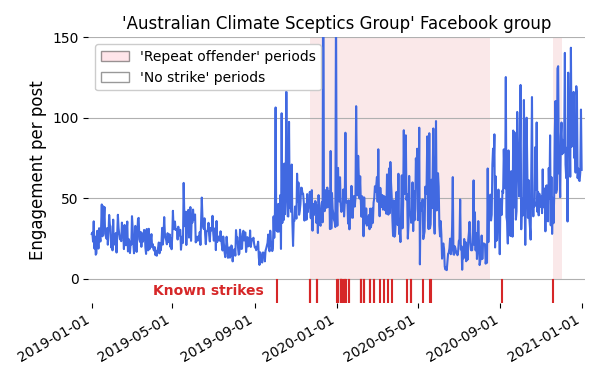
\includegraphics[scale=0.5]{./../figure/sf_example_timeseries.png}
\caption{
Average engagement (the sum of comments, shares, likes, ...) per post for the `Australian Climate Sceptics Group' Facebook group for each day in 2019 and 2020.
Each red line at the bottom represents the date of a known strike for this group according to the Science Feedback data. 
The areas shaded in red represent the `repeat offender' periods as defined by the ‘two strikes in 90 days’ rule.
}
\label{repeat_example_timeseries}
\end{figure}

To provide a general overview, we calculate the percentage change between the `repeat offender' and the `no strike' periods for each of the 256 Facebook accounts that have published at least one post during each period (see Figure \ref{repeat_vs_free_percentage_change}).\footnote{The percentage changes were calculated on the periods between January 1, 2019 and June 8, 2020. Because of the drop in engagement described further, the second semester of 2020 was excluded for its vastly diminished and not representative engagement level (see Figure \ref{repeat_average_timeseries}).}
The median percentage change is $-6\%$, and a Wilcoxon test shows that the values are not significantly different from zero (W = $16051$, p-value = $0.74$).

When we consider groups and pages separately, the results are different.
For the 238 Facebook groups, the percentage changes are not significantly different from zero (W = $13561$, p-value = $0.54$), with a median of $-3\%$, while for the 18 Facebook pages, the percentage changes are significantly different from zero (W = $21$, p-value = $0.0034$), with a median of $-43\%$.

\begin{figure}[!h]
\centering
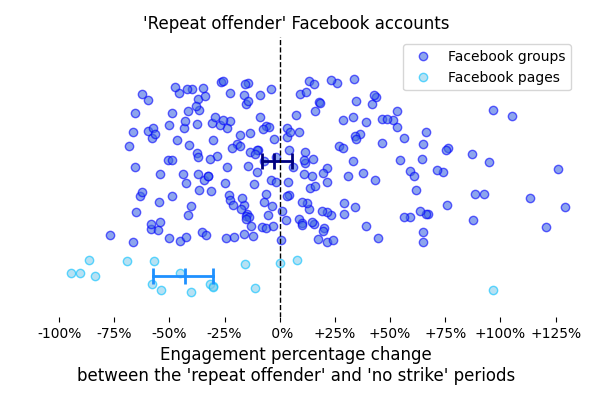
\includegraphics[scale=0.5]{./../figure/sf_repeat_vs_free_percentage_change.png}
\caption{
Percentage changes between the average engagement per post during the `repeat offender' periods and the `no strike' periods.
Each deep blue dot represents a Facebook group, and each light blue dot a Facebook page.
The bars show the medians for each set and their $90\%$ confidence intervals (the intervals are estimated using a bootstrap method).
The 256 `repeat offender' accounts represented here were identified by the Science Feedback data, and have published at least one post during each period.
}
\label{repeat_vs_free_percentage_change}
\end{figure}

To see whether the strikes would otherwise influence the repeat offenders accounts' engagement over time, we analyzed the total amount of engagement received by all the posts published by each of the 307 repeat offenders accounts for each day of the 2019-2020 period (Figure \ref{repeat_average_timeseries}). 
This metric, representing the total engagement generated by these accounts on Facebook (top panel), can be decomposed as the number of posts published each day (middle panel) times the average number of engagement per post (bottom panel).

The total engagement per day is stable from January to September 2019, however we observe a rise from September 2019 to June 2020. 
This rise is explained by the increase in activity of the misinformation accounts (with a doubling of the number of posts per day) while the engagement per post remained rather constant.
Around June 9, 2020, the total engagement metrics have massively dropped.
This decrease is entirely explained by a corresponding drop in engagement per post (Figure \ref{repeat_average_timeseries}).
This drop has cut the groups' engagement per post in half, but it was compensated by the fact that the overall activity of `repeat offender' has doubled between 2019 and 2020.
The engagement for `repeat offender' groups was thus reset by this intervention to its pre-pandemic level.

\begin{figure}[!h]
\centering
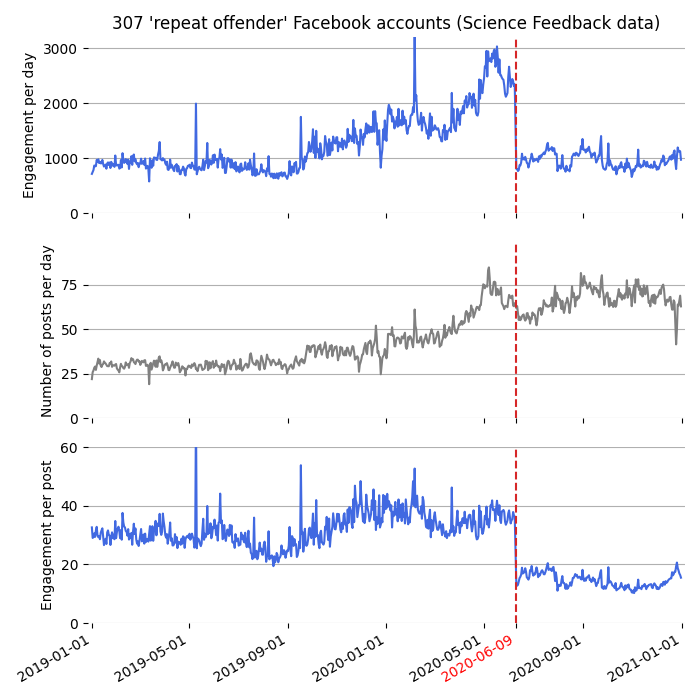
\includegraphics[scale=0.5]{./../figure/sf_average_timeseries.png}
\caption{
{\bf(Top panel)} Average engagement per day. 
{\bf(Middle panel)} Number of posts per day. 
{\bf(Bottom panel)} Average engagement per post. 
The dotted red line marks the date of June 9, 2020, when a sudden drop in engagement is observed.
The metrics were aggregated over the 307 `repeat offender' Facebook accounts identified by the Science Feedback data.
}
\label{repeat_average_timeseries}
\end{figure}

To further quantify this ‘June drop’, we calculated the percentage change in engagement for each account during a 30-day period before and after June 9, 2020 (Figure \ref{repeat_june_drop_percentage_change}). 
The median percentage change is $-43\%$, and most of the accounts (219 out of 289) experienced a decrease in engagement\footnote{A decrease in engagement on June 9, 2020 can be seen for the `Australian Climate Sceptics Group' in Figure \ref{repeat_example_timeseries} (the percentage change was $-60\%$ for this example).}.
A Wilcoxon test indicates that these percentage changes are significantly different from zero (W = $9012$, p-value = $4.6 \times 10^{-17}$).

Again the results differ between Facebook pages and Facebook groups.
While the percentage changes for the 271 groups are significantly different than zero (W = $7599$, p-value = $5.1 \times 10^{-17}$), with a median of $-45\%$,
the 18 pages appears to be not affected by the decrease (W = $73$, p-value = $0.61$), with a median percentage change of only $-5\%$.

\begin{figure}[!h]
\centering
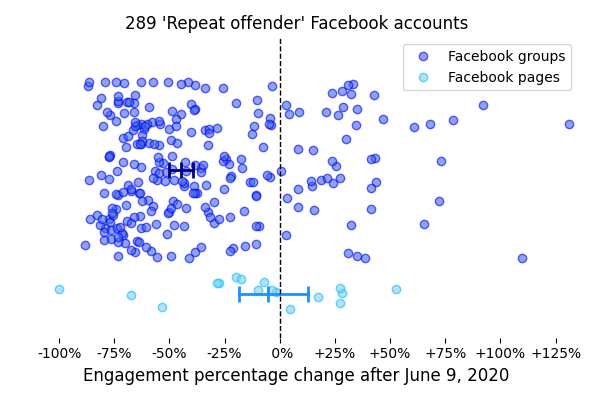
\includegraphics[scale=0.5]{./../figure/sf_june_drop_percentage_change.png}
\caption{
Percentage changes in the average engagement per post during a 30-day period before and after June 9, 2020. 
Each deep blue dot represents a Facebook group, and each light blue dot a Facebook page.
The bars show the medians for each set and their $90\%$ confidence intervals.
The 289 `repeat offender' accounts represented here were identified by the Science Feedback data, and have published at least one post one month before and one month after June 9, 2020.
}
\label{repeat_june_drop_percentage_change}
\end{figure}

To verify whether this drop was specific to this set of groups, we compared these dynamics to those of a control set of accounts consisting of Facebook pages and groups associated with established news outlets that did not publish misinformation.
No such drop in total or per post engagement metrics was observed around June 9, 2020 (see Supplementary Figure \ref{mainstream_average_timeseries}).

We can only explain such a massive change by a modification in how Facebook’s algorithm promoted the content from these groups starting on June 9, 2020.
While we did observe a relationship between the strike dates and a decrease in engagement for `repeat offender' pages, we observed no such link for `repeat offender' groups.
Hence it seems that Facebook only took action against these groups via this one-shot measure in June.

One limitation of the results described in this section is that we obtained the links labelled as `False' from only one fact-checking organization (Science Feedback), while Facebook partners with over 60 fact-checking organizations \citep{60factCheckingPartners}.
The true `repeat offender' periods could thus be longer than the ones inferred, potentially changing the magnitude of the ‘reduce’ effect.

\section{Investigating the reduce policy on accounts repeatedly sharing misinformation (Condor data)}

\subsection{Methods}

We used data from the Social Science One organization \cite{king2020new}, that builds partnerships between academia and private industries such as Facebook to share data and expertise. 
In July 2021, we had access to a new version of the Condor dataset \cite{messing2020facebook}, which contains all URLs shared publicly by at least 100 Facebook users between 2017 and 2021, as well as their fact-checking metadata. 
From this list, we extracted the 6,811 URLs that were shared in 2019 and 2020, that were fact-checked as `False' and whose country in which it was shared most frequently was either the USA, Canada, Great Britain or Australia.

We then replicated as closely as possible the methods used in the previous section. 
Using CrowdTangle, we thus collected all the posts that shared one of the false links between January 1, 2019 and December 31, 2020, and focused on the 706 Facebook accounts (671 Facebook groups and 35 Facebook pages) that spread at least 24 false links. 
Then we used CrowdTangle again to collect all the posts published by those accounts in 2019 and 2020. 
Because the Condor dataset contained the date of the first fact-check done on a URL, we were able to infer the `repeat offender' periods for each account and therefore conduct the same analysis as in the previous section.

Science Feedback being a third-party fact-checker working with Facebook, most of the URLs from Science Feedback were also contained in the Condor dataset ({\color{red}see Supplementary Figure X}). 
Thus an important part of the `repeat offender' groups and pages obtained from the Condor URLs were actually the same as the accounts analyzed previously ({\color{red}see Supplementary Figure X}). 
The point of this new analysis was to replicate the previous results with a more complete URL dataset and for this reason, we excluded the accounts whose engagement was already shown in the previous section. 
We thus show here the results for 503 `novel' accounts: 476 groups and 27 pages.

\subsection{Results}

\begin{figure}[!h]
\centering
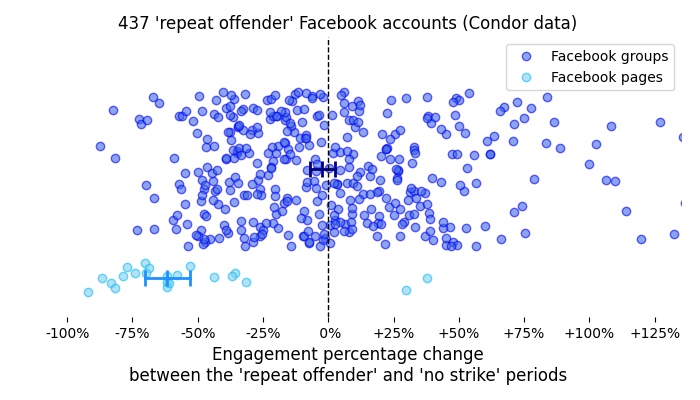
\includegraphics[scale=0.5]{./../figure/condor_repeat_vs_free_percentage_change.png}
\caption{
Same metric as on Figure \ref{repeat_vs_free_percentage_change}
The 437 `repeat offender' accounts represented here were identified by the Condor data, and have published at least one post during each period.
}
\label{condor_repeat_vs_free_percentage_change}
\end{figure}

Our first objective is to verify that the repeat offender policy was applied only to Facebook pages, and not to groups during the 2019-2020 period.
To do this, we calculate the percentage change in engagement between the `repeat offender' and the `no strike' periods for each of the 437 Facebook accounts that have published at least one post during each period (see Figure \ref{condor_repeat_vs_free_percentage_change}). 
The median percentage change is $-5\%$, and the values are not significantly different from zero (W = $46495$, p-value = $0.61$).

The changes in engagement are also different for the groups and the pages (Figure \ref{condor_repeat_vs_free_percentage_change}). 
The percentage changes for the 414 Facebook groups are not different than zero (W = $41561$, p-value = $0.57$), with a median of $-2\%$, while the values for the 23 Facebook pages are significantly different than zero (W = $29$, p-value = $0.00041$), and the median is $-62\%$.

\begin{figure}[!h]
\centering
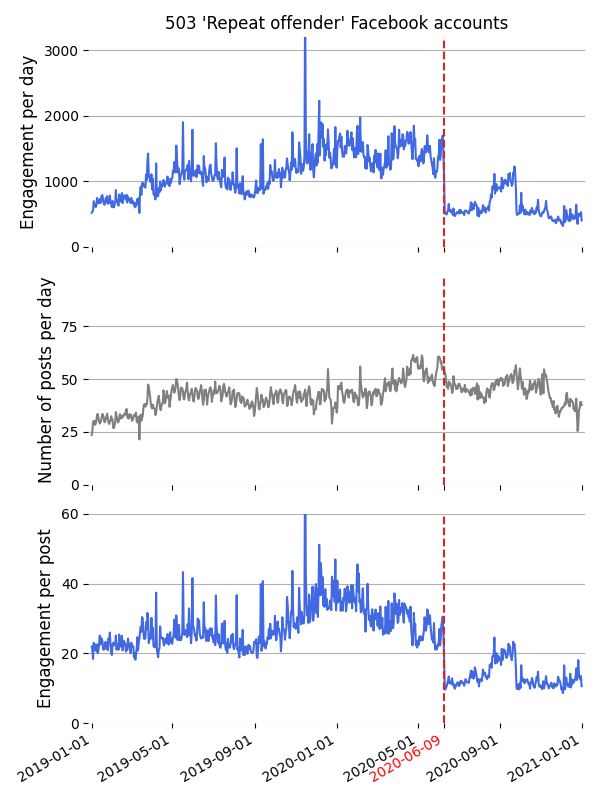
\includegraphics[scale=0.5]{./../figure/condor_average_timeseries.png}
\caption{
Same metrics as on Figure \ref{repeat_average_timeseries} aggregated over the 503 `repeat offender' Facebook accounts identified by the Condor data.
}
\label{condor_average_timeseries}
\end{figure}

As in the previous section, we then analyzed the engagement received by the 503 repeat offenders accounts in 2019 and 2020 (see Figure \ref{condor_average_timeseries}). 
The `novel' accounts replicated the slow rise in total engagement from September 2019 to June 2020, and the massive drop around June 9, 2020.
Again, we observe that this measure set the engagement for ‘repeat offenders’ groups back to its early 2019 level.

The percentage change in engagement was then calculated for each account during a 30-day period before and after June 9, 2020 ({Figure \ref{condor_june_drop_percentage_change}).
The median percentage change is $-26\%$, and $63\%$ of the accounts experienced a decrease in engagement, the results being a little more modest than what was found previously.
The values are still significantly different from zero (W = $42651$, p-value = $3.8 \times 10^{-5}$).

When tested separately, the percentage changes for the 442 groups are significantly different from zero (W = $37889$, p-value = $3.8 \times 10^{-5}$) and the median is $-27\%$, whereas the values for the 23 pages are not different from zero (W = $133$, p-value = $0.89$), with a median of $-2\%$.

\begin{figure}[!h]
\centering
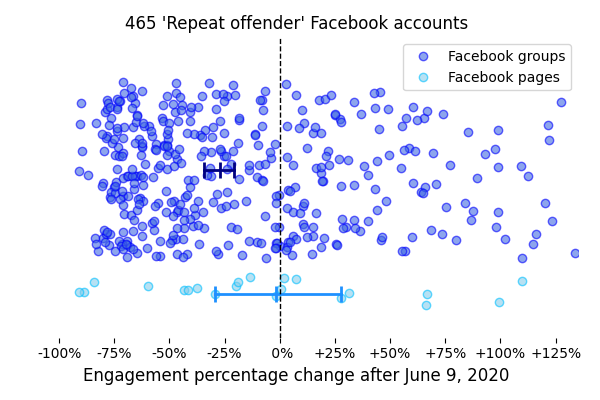
\includegraphics[scale=0.5]{./../figure/condor_june_drop_percentage_change.png}
\caption{
Same metric as on Figure \ref{repeat_june_drop_percentage_change}.
The 465 `repeat offender' accounts represented here were identified by the Condor data, and have published at least one post one month before and one month after June 9, 2020.
}
\label{condor_june_drop_percentage_change}
\end{figure}

To conclude, using a more complete dataset of `False' URLs and collecting new Facebook accounts, we replicated our previous findings. 
Indeed we again find a sudden decrease in engagement for repeat offender Facebook groups in June 2020, and a decrease in engagement following the publication of two false links for repeat offender Facebook pages.

One limitation of the results is that this king of analysis is rather indirect, as we relied on the strike dates to infer the `repeat offender' periods, and we cannot know for certain whether the pages investigated were actually under a `repeat offender' status. 
For example, one could imagine that the `two strikes in less than 90 days' rule may have changed over time, or that links fact-checked as `partly false' or `missing context' were also counted as strikes (only links fact-checked as `False' were taken into account in our analysis).
In the next section, we used a different methodology to collect pages for which we are sure that they are under `repeat offender' status.

\section{Investigating the reduce policy on pages declaring to be under `reduced distribution'} 

\subsection{Methods}

We noticed that two popular pages (`Mark Levin' and `100 Percent FED Up') have publicly shared a message claiming to be placed under `repeat offender' status with a screenshot as a piece of evidence.
To gather a list of such self-declared repeat offenders, we searched on CrowdTangle for posts published since January 1, 2020 with the following keywords:
\begin{itemize}
\item `reduced distribution' AND (`restricted' OR `censored' OR `silenced')
\item `Your page has reduced distribution'
\end{itemize}
For this we used the `/posts/search' endpoint of the API on November 25, 2020. 

We manually opened the resulting posts, and kept the ones which met the following criteria (see Figure \ref{reduce_example} top panel for an example):
\begin{itemize}
\item The post should include a screenshot of the Facebook notification.
\item In the screenshot, the Facebook notification should say: `Your page has reduced distribution and other restrictions because of repeatedly sharing of false news.'
\item In the screenshot, the name of the page should be visible.
\end{itemize}

Doing so, we obtained a list of 94 pages. 
We found only Facebook pages in this case, and no groups. 
A search using the terms `Your group has reduced distribution' did not yield any result.

To verify whether Facebook applied any restriction to these pages, we collected all the posts that these 94 pages have published between January 1, 2019 and December 31, 2020 from the CrowdTangle API using the `/posts' endpoint. 
The collection was run on January 11, 2021.
We were only able to collect data from 83 of these pages, as 11 were deleted from the CrowdTangle database since our search in November 2020. 
This highlights an important issue when studying misinformation trends on Facebook: some data disappears as accounts are deleted or changed to ‘private’.

The date of the last notification was used as the inferred start date of reduced distribution, when it appeared in the screenshot. 
When it was not visible, we used the date of the post as the inferred start date of reduced distribution. 

\subsection{Results}

\begin{figure}[!h]
\centering
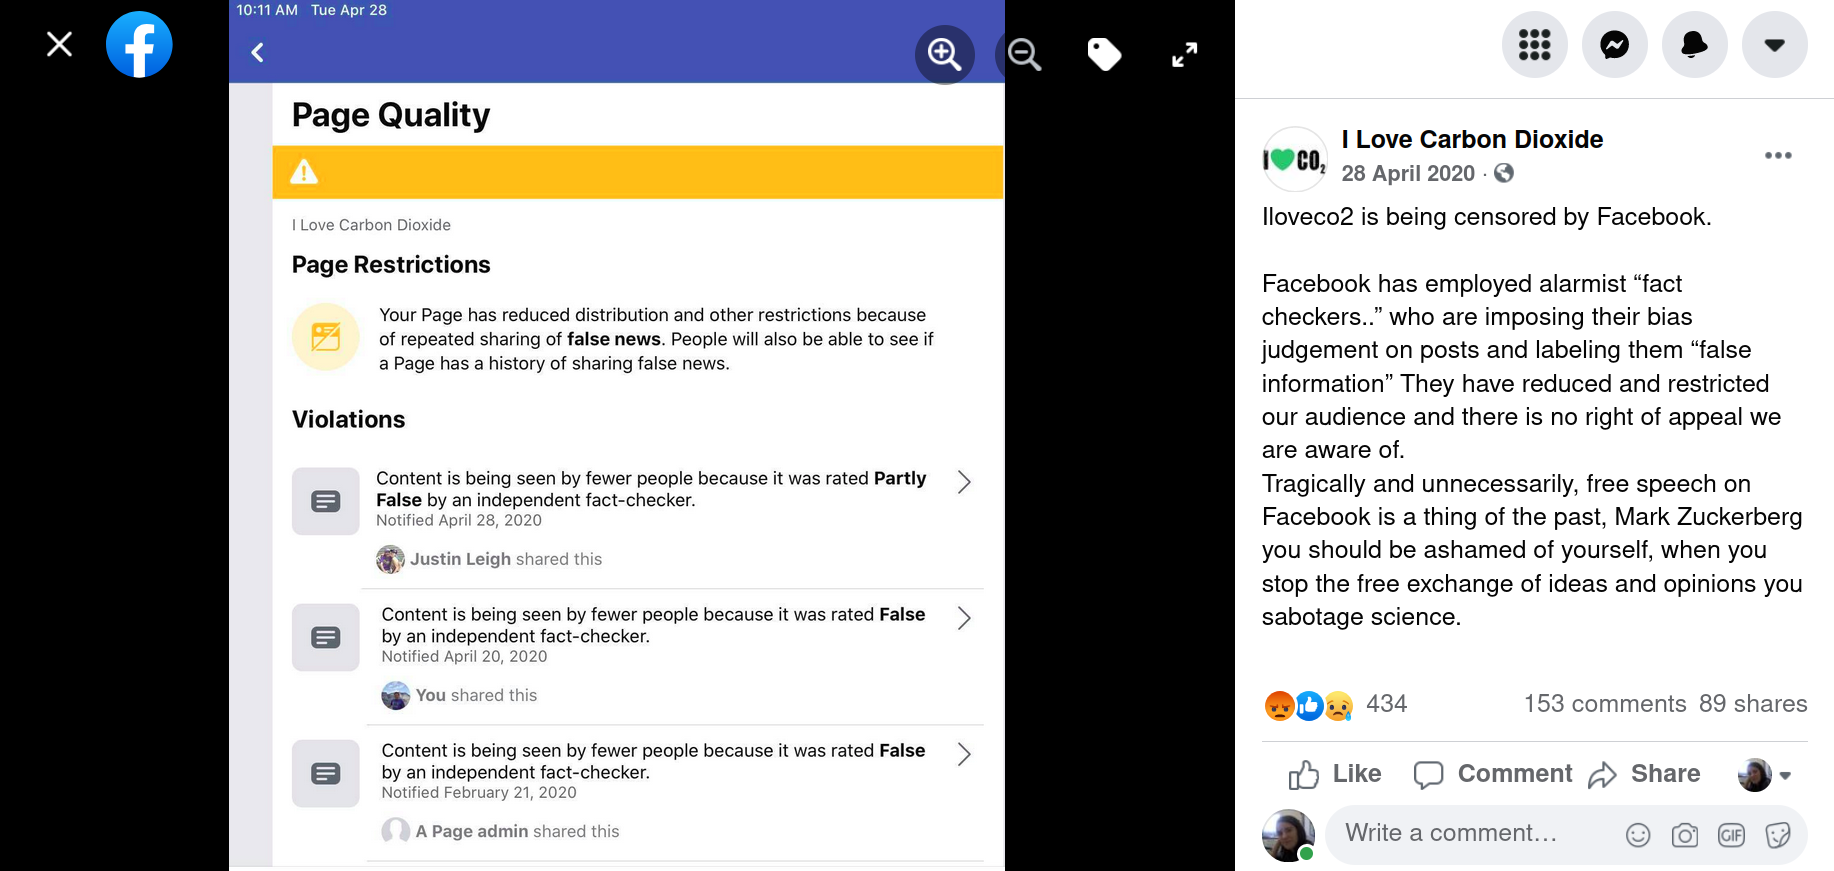
\includegraphics[scale=0.12]{./../figure/reduce_example_screenshot.png}
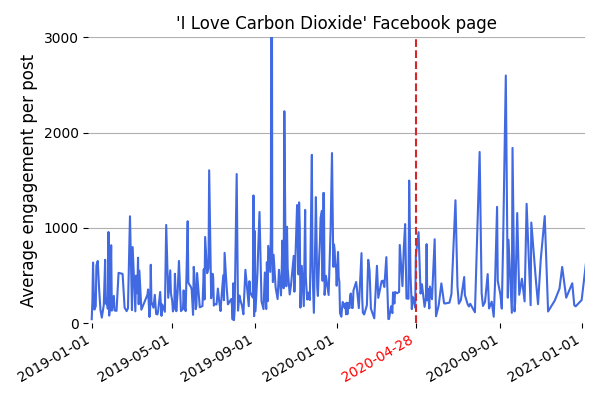
\includegraphics[scale=0.5]{./../figure/reduce_example_timeseries.png}
\caption{
{\bf(Top panel)} Screenshot of a \href{https://archive.is/ie4dR}{post from the `I Love Carbon Dioxide' Facebook page} sharing a `reduced distribution' notification from Facebook. 
{\bf(Bottom panel)} Average engagement per post for the “I Love Carbon Dioxide” page for each day in 2019 and 2020.
The dotted red line represents the reduced distribution start date.
}
\label{reduce_example}
\end{figure}

Figure \ref{reduce_example} shows a screenshot of the Facebook notification shared by the ‘I Love Carbon Dioxide’ page on April 28, 2020, and the average engagement per post of that page over the past two years. 
The engagement does not appear to be reduced after April 28, 2020. 
When we compare the engagement during a 30-day period before and after this date, the percentage change is $2\%$, indicating that the engagement is not affected by the `repeat offender' status.

To provide a general overview, we calculate the percentage change in engagement during a 30-day period before and after the reduced distribution start date for each of the 82 Facebook pages that published at least one post during each period (see Figure \ref{reduce_percentage_change}).
The median percentage change is $-24\%$, and a Wilcoxon test reveals that the percentage changes are significantly different from zero (W = $911$, p-value = $0.00026$).
We can thus suggest that the `reduced distribution' status is associated with a modest decrease in engagement.

\begin{figure}[!h]
\centering
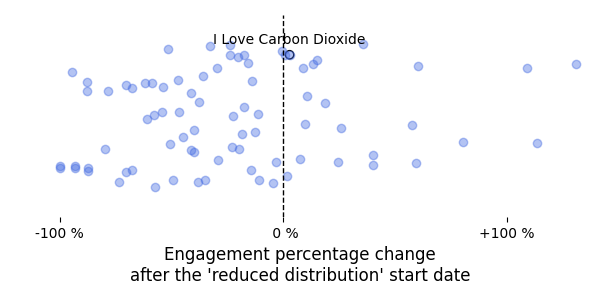
\includegraphics[scale=0.5]{./../figure/reduce_percentage_change.png}
\caption{
Percentage changes in average engagement per post during a 30-day period before and after the reduced distribution start date. 
Each dot represents a Facebook page. 
The bars show the median and its $90\%$ confidence interval.
The 82 `reduced distribution' pages represented here were identified because they shared a `reduced distribution' notification from Facebook in 2020.
}
\label{reduce_percentage_change}
\end{figure}
 
Finally, we verify whether an important drop in engagement also occurred in June 2020 for this set of Facebook pages.
When we compare the engagement metrics before and after June 9, 2020, the percentage changes are not significantly different from zero (W = $1093$, p-value = $0.055$), and the median percentage change is $3\%$.
This confirms that Facebook pages have most likely not been affected by the {\it reduce} measure implemented on June 9, 2020 and evidenced in the previous sections.

\section{Discussion}

Facebook, the most widely used social media platform in the world, has announced a series of measures to curb the spread of misinformation, notably by reducing the visibility of `repeat offenders', which are accounts that repeatedly share false information. 
However, the effects of the platforms' diverse policies to tackle misinformation remains understudied \citep{pasquetto2020tackling}. 
The present research article aims to contribute to filling this knowledge gap by verifying the application and measuring the consequences of Facebook's `reduce' policy on the targeted accounts' engagement metrics.

As a first step, we investigated the reach of 307 Facebook accounts (mainly groups) having repeatedly shared misinformation using a fact-checker's dataset. 
Sharing two false links over a three-month period is supposed to be penalized by a reduced visibility of the account's content. 
We did observe a significant decrease (median of $-43\%$) in the engagement per posts published by pages under a presumptive repeat offender status.
However, we find no evidence that this policy is leading to a significant decrease in engagement for Facebook groups.

{\color{red} ADD CONDOR RESULTS}
 
As a second step, we identified 83 Facebook pages which have shared a Facebook notification, indicating that their account was under reduced distribution.
The pages' engagement metrics were significantly lower after the date of the notification (median of $-24\%$), suggesting that the `reduced distribution' measure was indeed applied to the pages.
We noted that no group was found when searching for accounts sharing a reduced distribution notification, which confirms that the `repeat offender' policy is applied only to Facebook pages, and not to groups.

Although we observe a global reduction in engagement for `repeat offender' pages, there is a large heterogeneity across the different pages (see Figures \ref{repeat_vs_free_percentage_change}, \ref{condor_repeat_vs_free_percentage_change} and \ref{reduce_percentage_change}). 
The engagement of some popular pages have actually increased, such as the \href{https://www.facebook.com/TuckerCarlsonTonight/}{`Tucker Carlson Tonight' page} with a $38\%$ increase (from 104k to 143k interactions per post)  following the `reduced distribution' notification from Facebook. 
It is possible that this page compensated the reduce intervention of Facebook by a simultaneous gain of popularity, but a recent article points toward an alternative explanation. 
Some high-profile Facebook users such as celebrities, politicians and journalists might be exempted from the normal enforcement processes, according to company documents revealed by the Wall Street Journal \citep{WSJrevelations}.

By analyzing the time series of the repeat offenders’ engagement over the past two years, we also discovered a sudden drop affecting the groups around June 9, 2020.
For many groups, the decrease was quite drastic (up to $70\%$ - $80\%$), with a median drop in engagement of $45\%$.
The 18 Facebook pages from the first sample, as well as the 83 pages from the second sample, were not affected by this decrease.
This `June drop' does not correspond to any official communication by Facebook on that matter. 
It indicates that the company has very likely taken internal decisions that heavily impact the organic reach of repeat offenders' groups, in ways that differ from its stated policy against repeat offenders pages.
More transparency from Facebook would be needed to understand the nature and origin of this change. 
It would also bring clarity on how rules aimed at limiting the spread of misinformation are being enforced.

Facebook pages and groups have different purposes: pages are meant to be for official communication from the page administrators to a large audience, while groups are meant to foster interactions between users \citep{differenceGroupAndPage}. 
Pages are thus always public, while groups can be public or private.
Pages' posts can also be monetized and promoted.
Despite these differences, we have seen that both pages and groups are being used to share false news, and we actually found vastly more groups than pages when we identified the accounts spreading the most misinformation ({\color{red} add proportions?}). 
In the interest of curbing the spread of misinformation, applying its `repeat offender' policy to groups as well as to pages would help Facebook decrease the amount of misinformation in their users’ feeds. 

It is also not clear why only repeat offender Facebook groups, and not pages, saw their engagement reduced in June 2020.
Studies have highlighted that misinformation persists at high levels on Facebook and other platforms \citep{kornbluh2020new, resnick2018iffy}.
In the context of the COVID-19 pandemic, concerns rose about the amount of misinformation spreading on social media, including Facebook, and its potential harm to users \citep{johnson2020online}.
It is possible that such concerns have driven Facebook to apply a `quick fix' to decrease the engagement of posts shared in groups spreading misinformation and compensate for the absence of a repeat offender policy.
One should note that since the overall activity in these misinformation groups doubled between September 2019 and June 2020, the `June drop' has only succeeded in bringing the overall engagement level back to its early 2019 values (see Figure \ref{repeat_average_timeseries} top panel).

Online misinformation can be a threat to society, and the role that platforms can play via targeted interventions, has been the subject of intense debate over the past few years \citep{rogers2020deplatforming}. 
As a consequence, researchers \citep{mena2020cleaning, yaqub2020effects} and journalists \citep{FacebookPartisanBias, FacebookCivilityGrowth} have begun to monitor the actions that platforms take to tackle misinformation and their efficacy.
Given the facts that 1) false news go viral much faster than fact-checks can get published, 2) accounts that have shared misinformation in the past tend to keep sharing misinformation and 3) a small number of accounts is responsible for a large proportion of the misinformation being shared (at least regarding COVID-19 \citep{disinformationDozen}), acting against `repeat offenders' is likely to be one of the most effective interventions that platforms can make to protect their users against manipulation.

There is a critical need for further research to thoroughly verify and shed light on platforms' actions against misinformation. 
While our results provide information on the relative drop in engagement per post resulting from Facebook’s repeat offenders policy, more research is needed to quantify the impact of such policies on the overall prevalence of misinformation in users’ feeds.

%\begin{enumerate}[(1)]
%\item Group the authors per affiliation.
%\item Use footnotes to indicate the affiliations.
%\end{enumerate}

\bibliography{mybibfile}

\newpage

\beginsupplement

\textbf{SUPPLEMENTARY INFORMATION}

\section*{Engagement dynamics in 2019-2020 for a control set of accounts}

We compared the dynamics of the `repeat offender' accounts to those of a control set of accounts, which consisted of Facebook pages and groups associated with established news outlets that we expect to have a more stable pattern of publishing and represent the baseline journalistic activity.
To identify such a set, we used a report from NewsWhip \citep{NewsWhipReport} that identified the 10 media outlets that communicated the most during the early phase of the COVID-19 pandemic (first half of 2020), i.e., NBC, The Daily Mail, CNN, Fox News, The Independent, BBC, The New York Times, The Washington Post, Yahoo and The New York Post. 
We call this set `established news'; this label does not imply the trustworthiness of these news sources, but rather that they are very widely read and shared online. 
We searched the outlets' names on Facebook and created a list of 10 pages and six groups that displayed a verified `blue check'.
Using CrowdTangle, we collected all the posts published by these 16 accounts between January 1, 2019 and December 31, 2020.

\begin{figure}[!h]
\centering
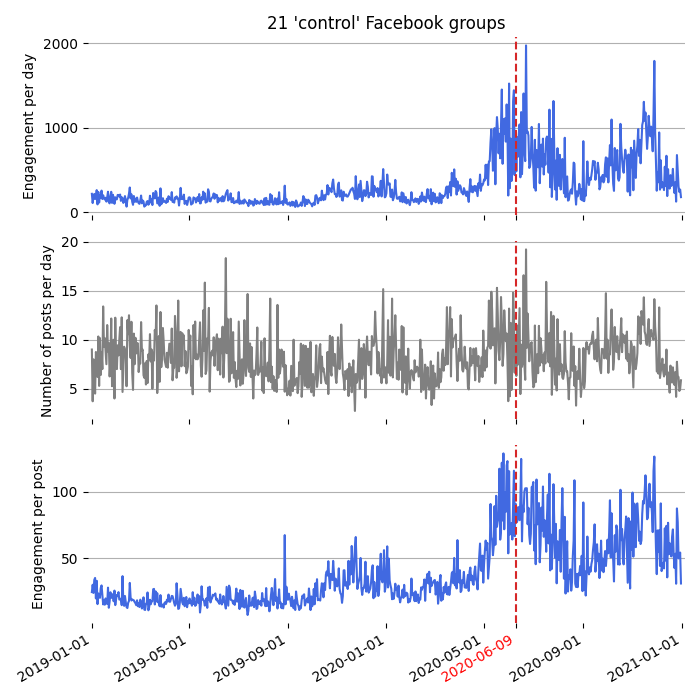
\includegraphics[scale=0.5]{./../figure/supplementary_mainstream_average_timeseries.png}
\caption{
Same metrics as on Figure \ref{repeat_average_timeseries} aggregated over the 16 Facebook accounts associated with a variety of `established news' outlets (NBC, The Daily Mail, CNN, Fox News, The Independent, BBC, The New York Times, The Washington Post, Yahoo and The New York Post).
}
\label{mainstream_average_timeseries}
\end{figure}

The average engagement aggregated for this set of accounts is presented in Figure \ref{mainstream_average_timeseries}.
Contrary to what we observe for the `repeat offender' accounts, there is no drop in total (upper panel) or per post (bottom panel) engagement around June 9, 2020 for the `established news' accounts. 
This observation further supports the hypothesis that the drop observed for the `repeat offender' groups is specifically targeted at these misinformation groups, and not a feature that broadly affected Facebook groups.
The number of posts per day per account is remarkably constant throughout the entire period, at around 55 posts per day per account (middle panel). 
The total engagement remained relatively constant during 2019, while we observe an increase in 2020, which peaked in early November 2020, corresponding to the American presidential elections. 
The sharp peak around Election Day is likely due to a change in behaviour of the audience that might have been actively seeking posts from established news outlets at that time, consistent with the `fly to quality' news effect observed at the start of the COVID-19 pandemic \citep{flyToQuality}.

\section*{Overlap between the different sets of repeat offender accounts}

In the two first methods, we used two different sources to get a list of False URLs fact-checked in 2019-2020, but there should be an overlap between these two lists. 
Indeed, Science Feedback is a third-party fact-checker partnering with Facebook \citep{sciencefeedbackFbPartner}, and the URLs fact-checked by Science Feedback were transfered to Facebook.
We can thus imagine that the list of URLs from Science Feedback would be included in the list from Condor.

However the only URLs that are in Condor are the ones shared by more than 100 users on Facebook, which excludes the less viral URLs fact-checked by Science Feedback.
Moreover, as Condor is one of the largest social science research dataset ever constructed, issues related to data quality, validity and fidelity are expected to be found \cite{messing2020facebook}.
For example it was recently revealed that the engagement data in Condor was only based on around half of the U.S. users and thus incomplete, because the views of the users that were not politically classified were not taken into account \citep{NYTrevelations}. 
Although this error should not impact the list of URLs we used in this article, other issues might have altered the list of False URLs, and that reason could also explain why some URLs from Science Feedback were excluded from the Condor list.

\section*{Characterization of the accounts studied} 

\end{document}
